%%%%% Background Information %%%%%

\chapter{Technical Background} \label{ch_background}

Before delving into this thesis' product, an overview of the involved technologies is given in this chapter: The described environment is implemented in ``Glamorous Toolkit'', which will be introduced in \ref{sc_gt}, using ``Moldable Development'' patterns (a concept introduced in \ref{sc_moldable}). Finally, as a teaching language, we've chosen ``Processing'' for which an overview is first given in \ref{sc_processing}.



\section{Processing} \label{sc_processing}

``Processing'' is a programming language consisting of a graphics \ac{API} built upon a mainstream language as a base. Development started between 1997 and 2004 at the MIT Media Lab as a continuation of the ``Design By Numbers`` project with the goal of creating a unified environment for teaching art students the fundamentals of programming as basis for creating digital, visual art.

While the original ``Design By Numbers'' integrated the language into an \ac{IDE}, having input and output side-by-side, it used its own, simplified programming language \cite{DBN01}. Processing's authors, Reas and Fry, based their language upon then popular and portable Java, removing much of the boilerplate required for object orientation, enhancing it with visual primitives and implicitly showing an output window, allowing for quick results (see figure \ref{fig_alpinerWanderweg}).

\begin{cfigure}[fig_alpinerWanderweg]{Example code (with Java syntax) and output}
\begin{minipage}{.5\textwidth}
\begin{code}
// Output canvas dimensions
size(200, 200);
// (Default white) square
rect(50, 50, 100, 100);
// Red inner rectangle
fill(255, 0, 0);
rect(50, 50 + 100 / 3, 100, 100 / 3);
\end{code}
\end{minipage}
\begin{minipage}{.45\textwidth}
\centering

\includegraphics[height=3cm]{alpinerWanderweg}
\end{minipage}
\end{cfigure}

Inside the \ac{IDE}, Processing code is compiled to Java bytecode and run inside the same \ac{JVM} as the \ac{IDE}. The Processing \ac{API} was thus provided in the form of compiled Java code and that hasn't changed for the official Processing \ac{IDE} to this day.

Apart from graphical primitives, Processing features an implicit event loop which allows for creating (interactive) animations within a dozen lines of code (see figure \ref{fig_jumpingBall}).

\begin{cfigure}[fig_jumpingBall]{Example code (with Python syntax) and four output frames}
\begin{minipage}{.5\textwidth}
\begin{code}
y = 50; dy = 0

# called once after global code
def setup():
    size(100, 200)

# called repeatedly for every frame
def draw():
    global y, dy
    background(192)
    circle(50, y, 50)
    y += dy; dy += 1
    if y > height - 25:
        dy = -0.9 * dy
\end{code}
\end{minipage}
\begin{minipage}{.45\textwidth}
\centering

\includegraphics[height=3cm]{ball1}

\includegraphics[height=3cm]{ball2}

\includegraphics[height=3cm]{ball3}

\includegraphics[height=3cm]{ball4}
\end{minipage}
\end{cfigure}

Reacting to input happens either by pulling state while painting a frame (implicit global variables such as \ct{mousePressed}, \ct{keyCode}, \etc) or by defining event handlers alongside \ct{setup} and \ct{draw} (such as \ct{mouseClicked(event)} or \ct{keyTyped(event)}).

Since Python has become the prevalent teaching language \cite{Cod20}, Processing has been extended with a Python mode which uses Python as a basis with the Processing \ac{API} being available by default and the animation loop still being implicit \cite{Pro25}.

As the official Processing \ac{IDE} remains implemented in Java, Processing's official Python mode uses the Jython library for compiling the code to Java Bytecode so that it can be run in the same way as Processing programs written in the original Java mode \cite{Jyt25}. This also gives access to most of Python's vast standard library, with the exception of a few modules which for speed were precompiled to native code for the various platforms and thus had to be rewritten for or left out of Jython.

In fact, as the \ac{JVM} is sufficiently generic to be the target for a wide variety of other languages, further modes for JavaScript\footnote{Based on the Rhino compiler from \archivedurl{https://rhino.github.io/}.} or R\footnote{Based on the Renjin interpreter from \archivedurl{https://renjin.org/}.} have been added.

This allows using Processing and its dedicated \ac{IDE} to be used as a starting point for programming and later seamlessly transitioning to the desired language such as pure Python, which remains part of the motivation for students: learning an ``actually useful'' language.

Since developers have started moving away from the \ac{JVM}, there are now several reimplementations of Processing such as p5.js for running Processing on top of JavaScript in a web environment\footnote{\emph{Cf.} \archivedurl{https://p5js.org/} and try it out at \url{https://editor.p5js.org/}.}, p5.py for running Processing in a pure Python environment\footnote{Requiring two additional lines: \ct{from p5 import *} at the top and \ct{run()} at the bottom; see \url{https://github.com/gromko/p5-python}.} or a version of Processing for microcontrollers such as Arduino\footnote{\emph{Cf.} \archivedurl{https://www.arduino.cc/education/visualization-with-arduino-and-processing/}.}. As of this thesis, a limited version for a Smalltalk environment is also available (see chapter \ref{ch_pa} and appendix \ref{app_api} for an \ac{API} overview).

In fact, when we started teaching programming in high schools classes, we initially ran our own \ac{IDE} based on web technologies and p5.js with custom error handling and support for live programming\footnote{This \ac{IDE} is still available at \archivedurl{https://software.zeniko.ch/ProcessingIDE.zip}. Note that it's targeted at \ct{mshta.exe} and as such runs best under Windows.} before changing to the official \ac{IDE} for its Python mode.

Our experience of working with Processing with ninth and tenth graders over the past decade has shown that it allows novice programmers to learn enough of the language within a month that they're able to write a clone of a game like ``Pong'', ``Flappy Bird'' or ``Geometry Dash'' as a group project. Feedback from the various student groups about this part of the computer science curriculum has always been positive to very positive (and remains so, as we'll see in chapter \ref{ch_practice}).

Reasons to use Processing are thus manyfold: Processing allows a top down approach starting at visual arts, which allows to motivate students with less interest in mathematics and natural sciences; Processing also quickly yields pleasant looking results, which also adds to initial motivation \cite{Chi23}; then it can be based on currently widely used languages such as Python, which allows using it as a stepping stone and makes it a `real' programming language in the eyes of novices; on the other hand, Processing itself is sufficiently unknown that even students already experienced with programming will have something new to discover; additionally, Processing has a large community sharing sketches and ideas which can be used as inspiration for both students and teachers; finally, its proven itself in our own experience over the years.



\section{Moldable Development} \label{sc_moldable}

``Moldable development'' is a term coined by Nierstrasz and G�rba \cite{Gir22,Nie24} for a collection of development patterns which should make it easier to understand a computer system by extending (`molding') it with views and features. The goal of moldable development is to quickly get feedback on code and objects being worked on so that a programmer can confidently make appropriate changes.

In traditional \acp{IDE}, a running system is inspected either through its source code or its live runtime objects. Available views (see \ref{ssc_ides}) are static and new views are added through non-trivial extensions. Moldable development asks for an environment in which a tool is more easily adaptable to data, making it simple to write either one-off throw-away views and tools but also allowing to refactor such throw-away code into reusable components when needed.

Moldable development is thus a form of exploratory programming (cf. \ref{ssc_exploration}) on live objects where tools, whether one-off or reusable, are created in a bottom up approach with immediate feedback available at every step.

In order to support this, a moldable environment must have extensibility in its core, allowing to register tools and views \eg through a simple code annotation of a few characters which the environment can use to detect and include it (instead of having to write a lot of configuration boilerplate and overhead which \ac{IDE} extensions meant for independent distribution usually involve).

One core pattern of moldable development is the ``Moldable Object'': Objects should be implementable incrementally with live object states and previously developed views remaining available throughout the whole process. An object consisting of little more than a data wrapper is thus extended with new functionality as it fits the available live data -- instead of designing an object on a clean slate or along tests. Exploration code can then be extracted into tests, ensuring that what worked once will continue to work. Extending objects iteratively based on actual needs ensures that they remain transparent and that code is cleanly separated.

Having a moldable environment also allows for working on code and documentation intertwined, similar to literate programming \cite{Knu84}. In contrast to literate programming where code has to be extracted first, in moldable development every code snippet should be runnable on its own and beside code and documentation also live results can be included. This allows a moldable environment to be used to either first document ideas and then add matching code but also to document progress or explain written code (which can then easily be extracted into a test case).

For students, such a ``Project Diary'' pattern could be used as a learning journal (similar to Microsoft OneNote\footnote{\emph{Cf.} \archivedurl{https://www.microsoft.com/de-ch/microsoft-365/onenote/digital-note-taking-app}.}), for project exploration (similar to Jupyter notebooks\footnote{\emph{Cf.} \archivedurl{https://docs.jupyter.org/}.}) or for project documentation. Another useful pattern for teaching is the ``Composed Narrative'' which visualizes object relations through side-by-side views tailored towards explaining a relation or interaction.



\section{Glamorous Toolkit} \label{sc_gt}

\acf{GT} is a fully programmable environment optimized for moldable development (see \ref{sc_moldable}), consisting of a Smalltalk \ac{VM} and runtime environment, a custom user interface and the source code of the Smalltalk code for everything running within. By default, it persists its entire state into a system image so that live objects don't have to be recreated at restart and may outlive their original source \cite{Gir23}.


\subsection{Smalltalk VM}

Smalltalk is a fully object oriented language based on message passing\footnote{One of many characteristics that Smalltalk shares with Java.} that was originally designed for educational use and as a consequence has rather minimalist syntax that is supposed to read more naturally, limiting the use of parentheses, aligning punctuation with natural language (using full stops to end a statement and semicolons to continue a statement by sending another message to the same object) and interweaving a message's name with its arguments\footnote{\emph{Cf.} \eg the \ct{#ifTrue:ifFalse} message in figure \ref{fig_annotated_view} where each argument follows part of the name. Note that these are not the argument's names, these are declared separatly in the definition of \ct{#ifTrue:ifFalse}.} \cite{Gol83}.

One potential issue for programmers experienced in ALGOL-68-derived languages is operator precedence, which in Smalltalk is limited for simplicity to just three different levels: (1) messages without arguments; (2) binary operators (which in contrast to mathematics and most other languages discussed in this thesis all have the same precedence and left associativity, and are of course also implemented as messages); and (3) all other messages.

At \ac{GT}'s core is the OpenSmalltalk Cog \ac{VM}\footnote{\emph{Cf.} \url{https://github.com/OpenSmalltalk/opensmalltalk-vm}.}. The Cog \ac{VM} is open sourced (MIT licensed) and shared with other Smalltalk based environments, in particular \ac{GT}'s predecessors (see \ref{ssc_gt_history}). Its source code is written in a subset of the Smalltalk language \cite{Ing97}, which is transpiled to C for performance and for using the various available C compilers to achieve cross-platform compatibility. As a consequence, \ac{GT} runs on Unix systems just as well as under Windows.

Smalltalk and the Cog \ac{VM} are highly reflective, allowing access to all but the most fundamental built-ins. In fact, all messages passed are primarily implemented in Smalltalk, but common operations can be forwarded to native code with a \ct{<primitive:...>} pragma annotation with only a fallback being provided in Smalltalk for when the native implementation fails. In particular, the execution context and the compiled bytecode of any message are available for inspection and modification. This allows users to customize the environment entirely to their liking.

For performance, the Cog \ac{VM} includes a \ac{JIT} for compiling methods called multiple times to native code on the fly \cite{Ope25}. More recently, for further optimizations, an adaptive optimizier called ``Speculative Inlining Smalltalk Architecture'' (SISTA) has been introduced by Cl�ment B�ra \cite{Ber17} which also allows to save the optimized methods into the image, thus persisting them between restarts of the environment. The bytecodes used for \ac{GT} are thus those proposed by B�ra and Miranda \cite{Ber14} and diverges to some extent from the original Smalltalk-80 bytecode format \cite[p.\,596]{Gol83}, in particular by enabling (more) multi-byte instructions which allow compilers inline more common objects and code.

With \ac{GT} being based on a Smalltalk \ac{VM}, Smalltalk is \ac{GT}'s primary language. Support for other popular languages such as Python, JavaScript or Java is however possible by connecting to an external runtime through the \ct{LanguageLink} protocol, \ie by passing serialized objects over sockets \cite{Fra24}.\footnote{The serialization format chosen is either JSON or the more compact binary representation ``MessagePack'' (see \archivedurl{https://msgpack.org/}).} Obviously, objects in the other runtime can't be persisted there, however transferred data and objects can be recreated from persisted objects within the Smalltalk \ac{VM}.


\subsection{Moldable Interface}

While Smalltalk and the \ac{VM} are inherited, the user interface has been written afresh based on the cross-platform Skia Graphics Engine which also powers most modern web browsers.\footnote{\emph{Cf.} \archivedurl{https://skia.org/docs/}.} Every window is rendered according to a dynamic rendering tree where every element involved (being a Smalltalk object) indicated how it wants to be layed out and the layout is recalculated for all size changes.

\begin{cfigure}[fig_gt_screenshot]{\ac{GT} with a live notebook page (left) and inspectable object view (right)}
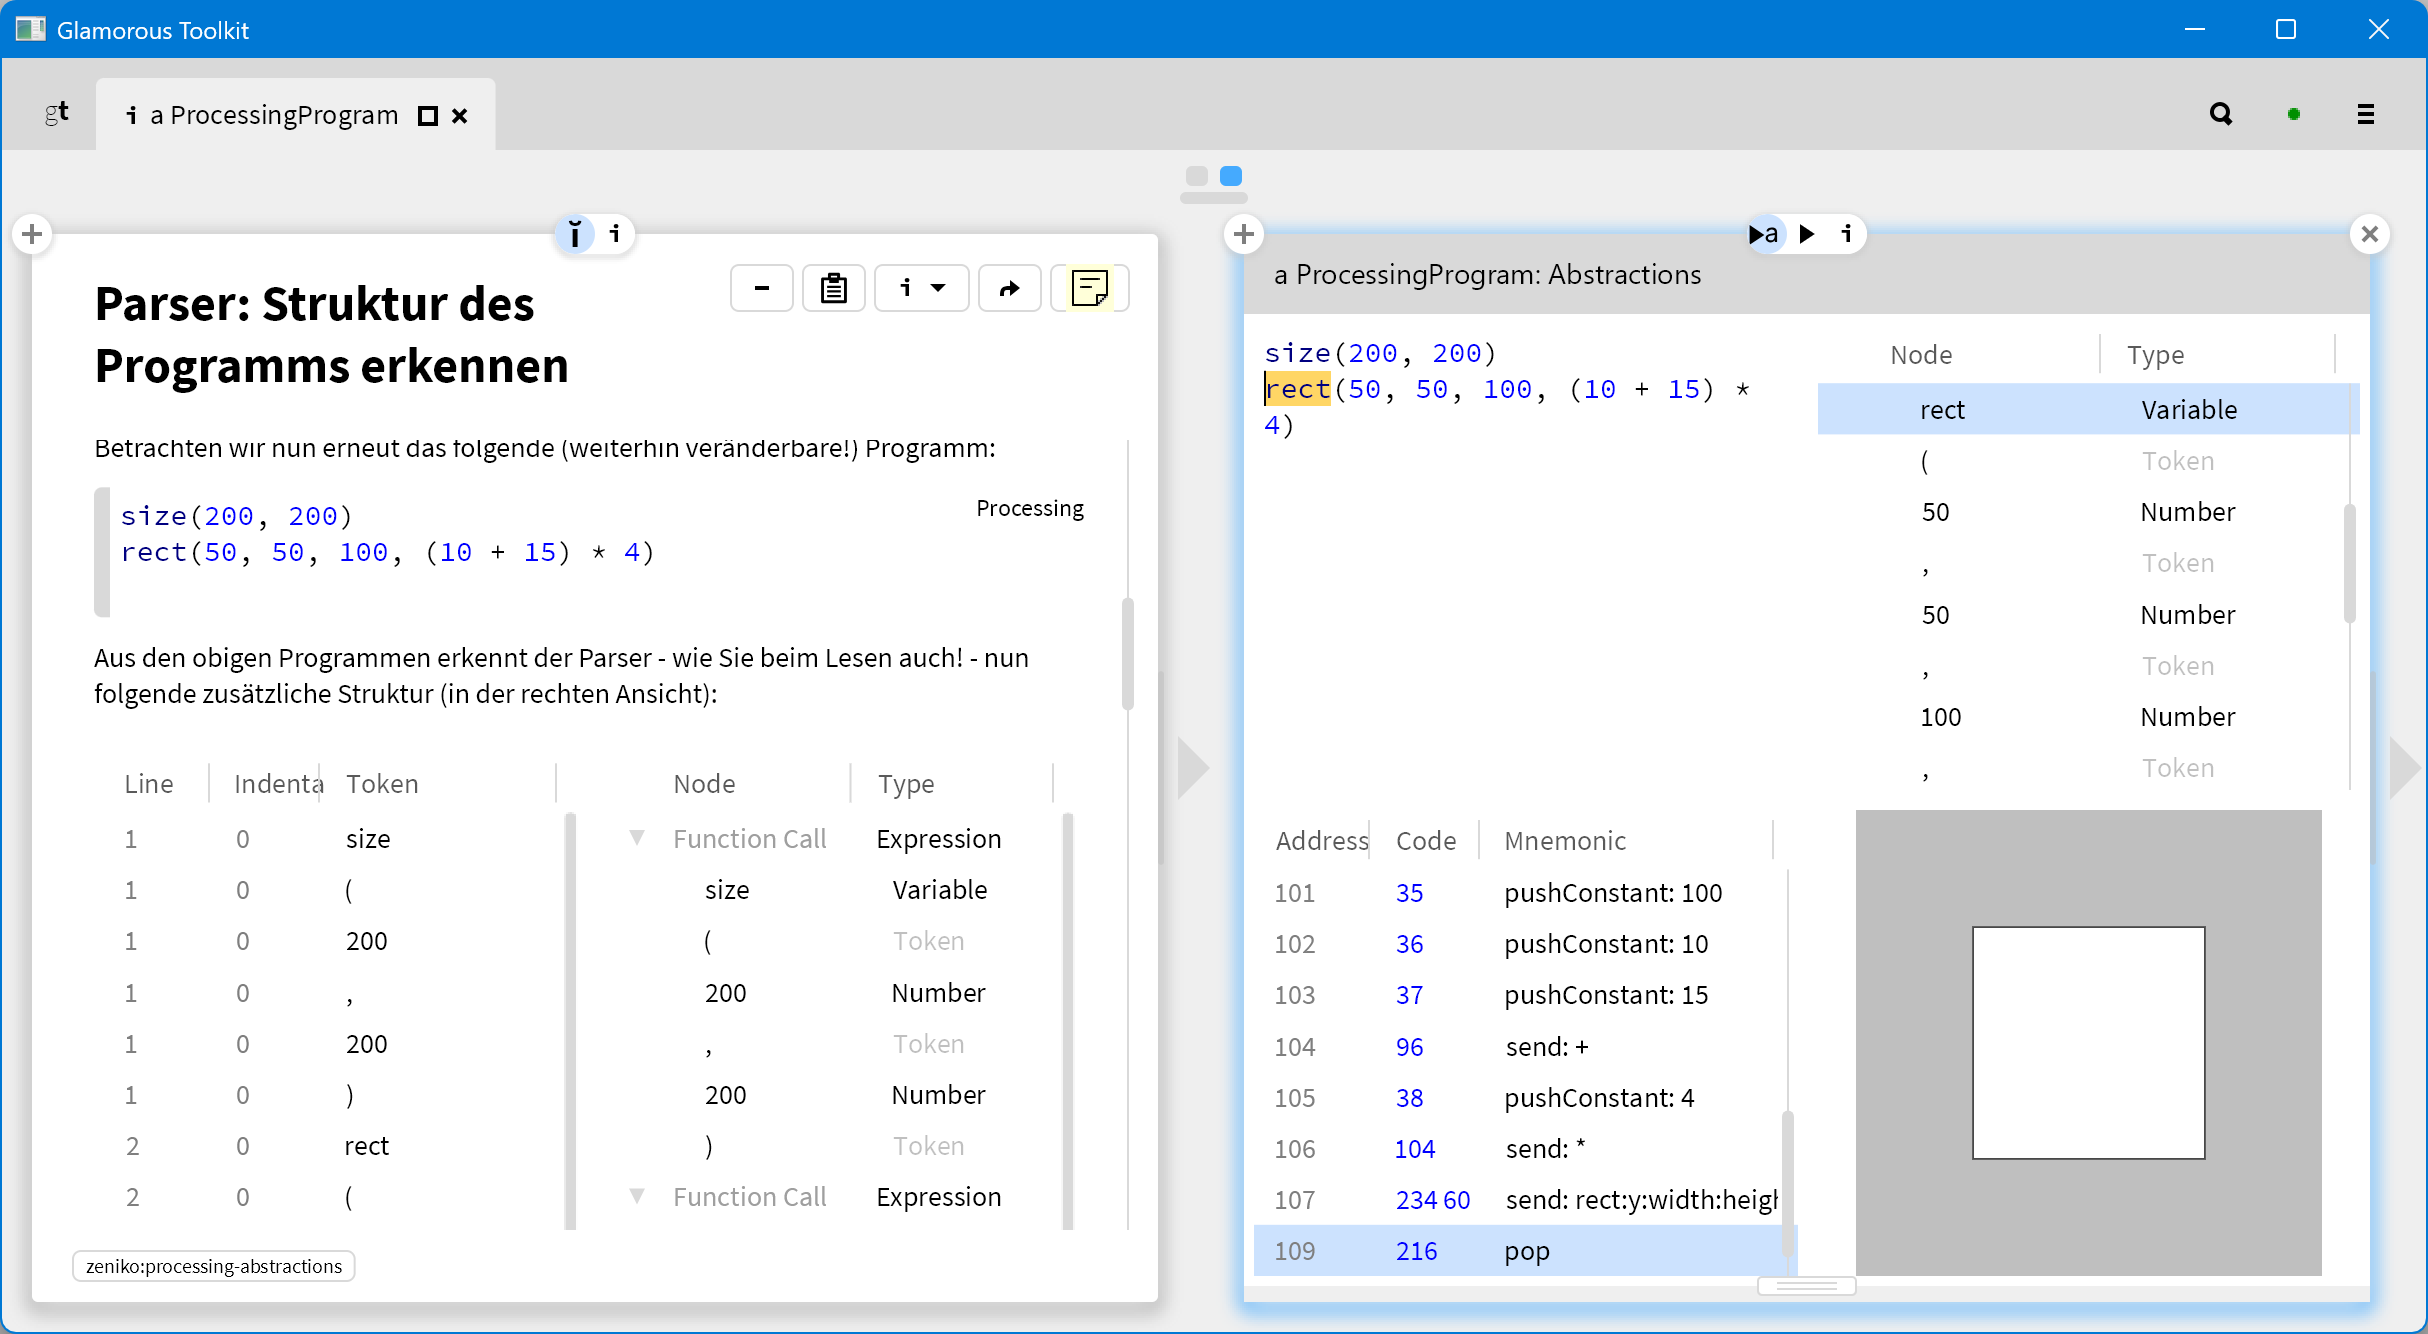
\includegraphics[width=.7\textwidth]{gt_screenshot}
\end{cfigure}

In its windows, \ac{GT} by default provides a tabbed interface which can show one of several tools: an object viewer, a notebook (dubbed ``Lepiter''), a code browser, a git interface and many more. While such tools are about as difficult to implement as an \ac{IDE} extension, the object viewer -- a tabbed interface itself -- is extended by simply annotating an object method which returns a \ct{GtPhlowView} object with the \ct{<gtView>} pragma as shown \eg in figure \ref{fig_annotated_view}).

\begin{cfigure}[fig_annotated_view]{Smalltalk source required for creating a custom view.}
\begin{code}
ProcessingCodeBase >> gtOutputFor: aView [
	<gtView>
	^ aView explicit
		title: 'Output' translated;
		priority: 40;
		stencil: [ (ProcessingRunner new
				limitTo: (self gtIsAnimation ifTrue: [ 30 ] ifFalse: [ 2 ]) seconds;
				run: self clone;
				canvas) asElement ]
]
\end{code}
\end{cfigure}

In this example, the element passed to the \ct{stencil:} message -- here the canvas resulting from running a Processing program -- could instead also be displayed inside a notebook page, with no annotations needed at all. Annotations are thus only required to allow \ac{GT} to discover messages of a certain type.

Similarly, methods annotated with \ct{<gtExample>} are considered tests and can be collectively inspected and run for a class or an entire package. This achieves several goals of moldable development: What starts as throw-away code can be extracted into a method, annotated and remains then permanently available for repeated testing. Examples are also includable by name in notebooks, where they do function as (tested and thus guaranteed working) examples for documentation.

Since one of \ac{GT}'s stated goals is to make systems explainable \cite{Gir23}, it provides ample packages for loading, transforming and visualizing data in various forms such as the SmaCC parser generator\footnote{\emph{Cf.} \archivedurl{https://refactory.com/smacc/}.}, a graph builder \cite{Mey06}, \etc, but also a built-in explanation system, allowing to visually connect arbitrary visual elements by annotating them.\footnote{In contrast to methods, objects are annotated by sending corresponding objects, in this case a \ct{GtExplainerTargetAptitude} or a \ct{GtExplainerExplanationAttribute} respectively.}.

What might take some getting used to: All Smalltalk code and all live objects are stored in \ac{GT}'s \ct{.image} file which is updated whenever \ac{GT} is closed with saving. This means that there are no source files outside of \ac{GT}'s interface. Synchronization of Smalltalk code thus happens best through \ac{GT}'s built-in git client. Preexisting notebook pages are also stored within one of \ac{GT}'s subdirectories. Users can however create new pages in the ``Local knowledge base''\footnote{By default, this is located in the \ct{lepiter} subdirectory of the user's documents or home folder.} which can be backed up separatedly and which are stored even when \ac{GT} is quit without saving. All notebook pages indicate where they're stored in their footer and can be moved between databases through that footer. This allows students to take an existing page from teaching material and move it locally where it's separately backed up, in case they later delete or update \ac{GT}.

\ac{GT} was thus chosen for its moldable environment: different views are quickly implemented and can be combined freely with interactions and updates between them.


\subsection{Bleeding Edge Issues}

The developers of \ac{GT} follow a trunk-only development style without release branches. This means that the release version changes almost daily, with new features being introduced gradually. This also means that subtle issues might be unexpectedly introduced in a release by or as a side-effect of some partially implemented feature. As a consequence, if \ac{GT} with an app is to be distributed, the best way to do this is by downloading the latest version, loading the app into it, verifying that it works and then distributing \emph{this known good} image.

When \ac{GT} is used heavily, occasionally some lesser tested code paths might be hit. We've occasionally had some modifier keys apparently lock up, requiring app switching to get keyboard shortcuts working again; we've sometimes hit a cascade of error messages, spawning dozens of debug windows which had to be closed without other consequences; and occasionally \ac{GT} seemingly stopped responding, with even the \ct{Ctrl+.} keyboard shortcut not interrupting the running code (luckily, code modifications are backed up and restoreable through the ``Code changes'' tool). Most of these are small annoyances which more restrained users -- such as students -- shouldn't encounter often.

Finally, \ac{GT} is mainly developed under macOS and makes some platform assumptions with relation to its host operating system. This isn't noticeable when working purely within \ac{GT} but occasionally shows at its seams, with external executables not being located reliably for establishing a link to other runtimes\footnote{\emph{Cf.} GitHub issues \href{https://github.com/feenkcom/gtoolkit/issues/4608}{feenkcom/gtoolkit\#4608} for Linux and \href{https://github.com/feenkcom/gtoolkit/issues/4633}{feenkcom/gtoolkit\#4633} for Windows.}, knowledgebase names containing path separators\footnote{Which can be worked around by renaming the database, see GitHub issue \href{https://github.com/feenkcom/gtoolkit/issues/3036}{feenkcom/gtoolkit\#3036}.}, or pasting source code from third party apps leading to visual bugs in \ac{GT}'s code editor.\footnote{This applies under Windows, see GitHub issue \href{https://github.com/feenkcom/gtoolkit/issues/4634}{feenkcom/gtoolkit\#4634}.} We'd assume that most of the reported issues could have been fixed at the time of reading, though.


\subsection{Historical Remarks} \label{ssc_gt_history}

Smalltalk environments have been image-based and resumable since the early days in the 1970s, when Alan Kay sketched out the original Smalltalk which he eventually standardized at Xerox into Smalltalk-80. Based on a Smalltalk-80 \ac{VM} by Apple, Ingals, Kay \etal started developing a new \ac{VM} and development environment which had the goal to also be customizable by non-programmers \cite{Ing97}: ``Squeak'' inherited its built-in capabilites for live and exploratory coding from the original Smalltalk and its back to this point that \ac{GT}'s heritage is tied directly.

While Squeak was further developed at Walt Disney Media Labs and among others included in the ``One Laptop per Child'' laptops, it remained a niche product -- likely due to missing interoperability between the live environment inside its \ac{VM} and outside code. Still, Squeak and its later fork Pharo continued being worked on and were actively being used in academia and related spin-offs. Eventually, a team around Tudor G�rba -- including this thesis' supporter Oscar Nierstrasz -- set out to implement their idea of a moldable environment on the basis of Pharo, thus creating \ac{GT} \cite{Fee25}. Version 1.0 has been released in 2023 and is still being actively worked on.

\ac{GT} thus has an illustrious lineage and has achieved support for many concepts asked for by literature: It's a moldable environment, supports a clean object-oriented language, allows for live and exploratory programming, still remains comparatively manageable and -- particularly relevant for this thesis -- allows for reflection at various levels, including for every object access to its method's source code, its compiled form and even its memory layout inside its \ac{VM}.
